\documentclass[a4paper,11pt]{article}

% Kodovani (cestiny) v dokumentu: utf-8
%\usepackage[cp1250]{inputenc}	% Omezena stredoevropska kodova stranka, pouze MSW.
\usepackage[utf8]{inputenc}	% Doporucujeme pouzivat UTF-8 (unicode).

\usepackage[margin=2cm]{geometry}
\newtoks\jmenopraktika \newtoks\jmeno \newtoks\datum
\newtoks\obor \newtoks\skupina \newtoks\rocnik \newtoks\semestr
\newtoks\cisloulohy \newtoks\jmenoulohy
\newtoks\tlak \newtoks\teplota \newtoks\vlhkost

\jmenopraktika={Fyzikální praktikum 3}
\jmeno={Lukáš Lejdar}
\datum={6. května 2025}
\obor={F}
\skupina={Út 14:00}

\cisloulohy={4}
\jmenoulohy={Studium termoelektronové emise}

%%%%%%%%%%% Uzitecne balicky:
\usepackage[czech]{babel}

\usepackage{graphicx}
\usepackage{amsmath}
\usepackage{xspace}
\usepackage{url}
\usepackage{indentfirst}
\usepackage{wrapfig}
\usepackage{xcolor}
\usepackage{subfig}
\usepackage{subcaption}
\usepackage{enumitem}
\usepackage{tikzsymbols}
\usepackage{newfloat}

\DeclareFloatingEnvironment[fileext=lof]{graph}
\captionsetup[graph]{labelformat=simple, labelsep=colon, name=Graf}

%%%%%% Zamezeni parchantu:
\widowpenalty 10000 \clubpenalty 10000 \displaywidowpenalty 10000
%%%%%% Parametry pro moznost vsazeni vetsiho poctu obrazku na stranku
\setcounter{topnumber}{3}	  % max. pocet floatu nahore (specifikace t)
\setcounter{bottomnumber}{3}	  % max. pocet floatu dole (specifikace b)
\setcounter{totalnumber}{6}	  % max. pocet floatu na strance celkem
\renewcommand\topfraction{0.9}	  % max podil stranky pro floaty nahore
\renewcommand\bottomfraction{0.9} % max podil stranky pro floaty dole
\renewcommand\textfraction{0.1}	  % min podil stranky, ktery musi obsahovat text
\intextsep=8mm \textfloatsep=8mm  %\intextsep pro ulozeni [h] floatu a \textfloatsep pro [b] or [t]

% Tecky za cisly sekci:
\renewcommand{\thesection}{\arabic{section}.}
\renewcommand{\thesubsection}{\thesection\arabic{subsection}.}
% Jednopismenna mezera mezi cislem a nazvem kapitoly:
\makeatletter \def\@seccntformat#1{\csname the#1\endcsname\hspace{1ex}} \makeatother
%
\newcommand{\vsn}[4]{\ensuremath{#1 =} #2(#3)\,#4}
\newcommand{\vrn}[6]{\ensuremath{#1 =} (#2 $\pm$ #3)\,#4 ($p=$ #5\,\%, $\nu=$ #6)}

\newcommand*\circled[1]{\tikz[baseline=(char.base)]{
		\node[shape=circle,draw,inner sep=1pt] (char) {#1};}}

%%%%%%%%%%%%%%%%%%%%%%%%%%%%%%%%%%%%%%%%%%%%%%%%%%%%%%%%%%%%%%%%%%%%%%%%%%%%%%%
% Zacatek dokumentu
%%%%%%%%%%%%%%%%%%%%%%%%%%%%%%%%%%%%%%%%%%%%%%%%%%%%%%%%%%%%%%%%%%%%%%%%%%%%%%%

\begin{document}

\thispagestyle{empty}

{
\begin{center}
\sf 
{\Large Ústav fyziky a technologií plazmatu Přírodovědecké fakulty Masarykovy univerzity} \\
\bigskip
{\huge \bfseries FYZIKÁLNÍ PRAKTIKUM} \\
\bigskip
{\Large \the\jmenopraktika}
\end{center}

\bigskip

\sf
\noindent
\setlength{\arrayrulewidth}{1pt}
\begin{tabular*}{\textwidth}{@{\extracolsep{\fill}} l l}
\large {\bfseries Zpracoval:}  \the\jmeno & \large  {\bfseries Naměřeno:} \the\datum\\[2mm]
\large  {\bfseries Obor:} \the\obor  \hspace{40mm}  {\bfseries Skupina:} \the\skupina %
&\large {\bfseries Testováno:}\\
\\
\hline
\end{tabular*}
}

\bigskip

{
\sf
\noindent \begin{tabular}{p{4cm} p{0.6\textwidth}}
\Large  Úloha č. {\bfseries \the\cisloulohy:} \par
\smallskip
&\Large \bfseries \the\jmenoulohy  \\[2mm]
\end{tabular}
}

\vskip1cm


\section{Úvod}

Cílem úlohy je zjistit výstupní práci elektronů wolframového vlákna měřením termoemisního proudu o ověřit rovnice popisující Schottkyho efekt z voltampérové charakteristiky urychlovacího napětí. 

\section{Teorie}

\subsection{Termoemise}

Elektrony ve vodivostním páse mohou uniknout ven z materiálu pouze tehdy, když jejich rychlost ve směru osy $x$ překoná výstupní práci $ w \ge m_e v_{x,\text{min}}^2 / 2 $ 

\begin{equation}
 \frac{1}{2} m_e v_x'^2 = \frac{1}{2} m_e v_x^2 - w
\end{equation}

Za běžných podmínek elektrony nemají dostatek energie na překročení potenciálové bariéry, ale je možné jim ji dodat třeba zahříváním látky na vysokou teplotu. Pro výpočet hustoty takového termoemisního proudu integrujeme rychlostní rozdělení uvnitř vodiče přes všechny elektrony s rychlostí $v_x > v_{x,\text{min}}$.

\begin{equation}
 j = \int_{-\infty}^{\infty} \int_{-\infty}^{\infty} \int_{ v_{x,\text{min}} }^{\infty} e v_x n(\vec{v}) dv_x dv_y dv_z
\end{equation}

\noindent
Transformací proměnných $ v_x' dv_x' = v_x dv_x $ dostáváme

\begin{equation}
 j = \int_{-\infty}^{\infty} \int_{-\infty}^{\infty} \int_{ 0 }^{\infty} e v_x' n(\vec{v}) dv_x' dv_y dv_z
\end{equation}

\noindent
a protože proud se nemění po překročení bariéry, můžeme ho také vyjádřit pomocí rychlostního rozdělení $n'$ vně materiálu

\begin{equation}
 j = \int_{-\infty}^{\infty} \int_{-\infty}^{\infty} \int_{ 0 }^{\infty} e v_x' n'(\vec{v}') dv_x' dv_y dv_z,
\end{equation}

\noindent
odkud 

\begin{equation}
n'(\vec{v}') =  n(\vec{v})
\end{equation}

\noindent
Na termoemisním proudu se budou podílet jen elektrony s vysokou energií v rámci rozdělení $ n $ a tam ho můžeme aproximovat jako

\begin{equation}
 n'(\vec{v}') = \frac{2 m_e^3 }{h^{3}} \exp\left( - \frac{m_e(v_x^2 + v_y^2 + v_z^2)}{2kT} + \frac{\mu}{kT} \right),
\end{equation}

\noindent
kde $ \mu $ je chemický potenciál uvnitř látky. Dosazením vztahu (1) dostáváme

\begin{equation}
n'(\vec{v}') = \frac{2 m_e^3 }{h^{3}} \exp \left( \frac{\mu - w}{k T} \right) \exp\left( - \frac{m_e(v_x'^2 + v_y^2 + v_z^2)}{2kT} \right),
\end{equation}

\noindent
takže rychlostní rozdělení elektronů vně by mělo být přibližně Maxwellovo o teplotě stejné jako uvnitř materiálu. Celkový proudu potom získáme provedením integrálu (4), který vede na Richardson – Dushmanovu rovnici

\begin{equation}
I_{\text{nas}} = B T^2 \exp\left(- \frac{w}{kT} \right)
\end{equation}

\noindent
kde $ B $ je konstanta zahrnující povrch katody a ostatní konstanty. Wolframovou Katodu budeme v praktiku zahřívat žhavícím proudem $ I_{f} $ přičemž víme, že odpor katody $ R_t $ závisí na teplotě $ t $ (ve stupních Celsia) v prvním přiblížení jako

\begin{equation}
\frac{U_f}{I_f} = R_t = \frac{\rho d}{ S} (1 + \alpha t)
\end{equation}

\noindent
kde $ \rho = 4.89 \cdot 10^{-8} \ \Omega  $m , d je délka vlákna, $ S $ je průřez vlákna, $ d / S = 7.76 \cdot 10^{6} \ \text{m}^{-1} $ a $ \alpha = 4.83 \cdot 10 ^{-3} \text{ K}^{-1} $ je teplotní součinitel odporu.

\subsection{Schottkyho efekt}

Pokud na katodu přivedeme vnější elektrické pole o intenzitě $ E $ směřující dovnitř, tak dojde k superpozici potenciálů a výstupní práce se sníží o hodnotu

\begin{equation}
 w_p = \sqrt{ \frac{e E^{3}}{4 \pi \varepsilon_0}}
\end{equation}

\noindent
a tedy nová hodnota $w'$ je

\begin{equation}
w' = w - w_p = w - \sqrt{ \frac{e E^{3}}{4 \pi \varepsilon_0}}
\end{equation}

\noindent
Dosazením do Richardsonovy – Dushmanovy rovnice dostáváme

\begin{equation}
    I_{\text{nas}}' = BT^2 \exp - \frac{w'}{kT}  = I_{\text{nas}} \exp \frac{w_p}{kT}
\end{equation}

 
\section{Postup měření}

Zapojení měřící aparatury je podle obrázku 1. Wolframové vlákno je umístěné do odvzdušněné elektronky a teče skrz něj proud $ I_f $, který můžeme regulovat zdrojem PS1. Emitované elektrony vyletují do všech stran, ale ty které dopadnou na anodu na druhé straně elektronky jsou zachyceny a měříme je jako anodový proud $ I_a $. Množství zachycených elektronů je možné buď dopomoct nastavením kladného napětí $ U_a $  na anodě, aby elektrony přitahovala, nebo záporně, které překonají jen ty elektrony, které mají složku kinetické energie směrem k anodě větší něž napětí $ e U_a $ 

\begin{equation}
e U_a \le  \frac{1}{2}m v_z^2  = E_k
\end{equation}

\noindent
Proud $ I_a $, který naměříme je potom podle vztahů (4) a (6) pro energetické elektrony daný jako

\begin{equation}
I_a = I_0 \exp \left( {\frac{e U_a}{kT}} \right)
\end{equation}

V experimentálním uspořádání je Wolframové vlákno zatočené do spirály o průměru$  2r = 0.09 $ mm, takže intenzitu elektrického pole v jejím okolí budeme aproximovat polem válcového kondenzátoru o vnějším poloměru vzdálenosti anody $ R = 17 $ mm. Pro přesnější určení se do vztahu přidal ještě faktor $ (L - D) / D $

\begin{equation}
E = U_a \frac{L - D}{D} \frac{1}{r \ln (R / r )}
\end{equation}

\noindent
kde $ D $  je vzdálenost anody od žhavené katody a $ L $  je vzdálenost anody od rovinné studené katody. 



\begin{figure}[htpb]
    \centering
    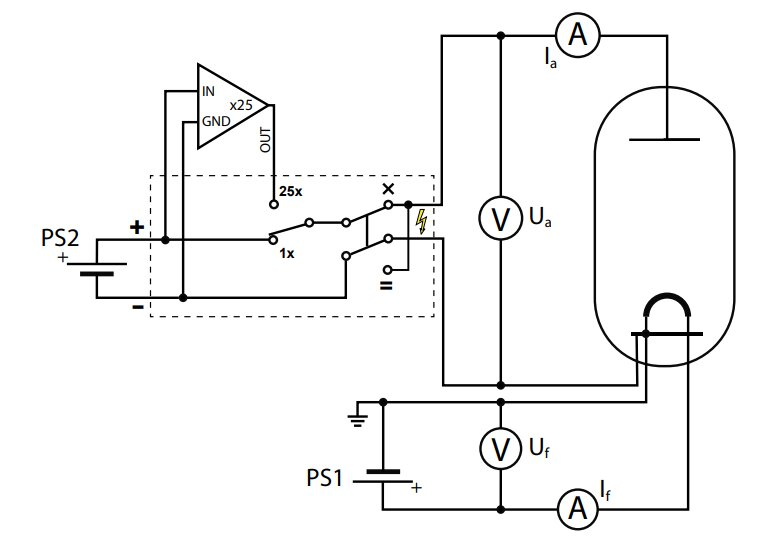
\includegraphics[width=0.7\textwidth]{zapojeni.jpg}
    \caption{Elektrické schéma zapojení diody pro studium efektu termoemise.}
\end{figure}

\newpage

\section{Výsledky měření}

\subsection{Závislost anodového proudu na anodovém napětí}

Aparaturu jsem zapojil podle obrázku (1) a zkontroloval, že všechny ovládací prvky fungují správně. Před měřením je potřeba nejdřív vlákno nažhavit, takže jsem nastavil žhavící proud na $ I_f = 1.92 $ A a počkal přibližně 10 minut. Po nažhavení vlákna jsem po malý krocích změřil závislost anodového proudu $ I_a $  na anodovém napětí v rozmezí $ U_a \in [-5, 500] $ a to stejné udělal ještě pro žhavící proud $ I_f = 1.98 $ A. Obě závislosti jsou uvedené v grafech 1 a 2, kde je vidět, že se anodový proud ustálí kolem 20 V a pak pomalu roste kvůli Schottkyho efektu. Grafy 3 a 4 vykreslují logaritmickou závislost proudu na napětí v oblasti záporného anodového napětí, které jsem fitoval podle zlogaritmováním vztahu (14) a ze sklonu získál teplotu $ T $, která je uvedena pod grafy. Se zjištěnou teplotou už bylo možné fitovat změřenou závislost v oblasti vyšších napětí vztahem (12) ze kterého jsem získal nasycené termoemisní proudy $ I_{\text{nas}} $.

\begin{table}[h]
    \captionsetup{type=graph}
    \begin{minipage}{.45\linewidth}
        \centering
        % GNUPLOT: LaTeX picture with Postscript
\begingroup
  \makeatletter
  \providecommand\color[2][]{%
    \GenericError{(gnuplot) \space\space\space\@spaces}{%
      Package color not loaded in conjunction with
      terminal option `colourtext'%
    }{See the gnuplot documentation for explanation.%
    }{Either use 'blacktext' in gnuplot or load the package
      color.sty in LaTeX.}%
    \renewcommand\color[2][]{}%
  }%
  \providecommand\includegraphics[2][]{%
    \GenericError{(gnuplot) \space\space\space\@spaces}{%
      Package graphicx or graphics not loaded%
    }{See the gnuplot documentation for explanation.%
    }{The gnuplot epslatex terminal needs graphicx.sty or graphics.sty.}%
    \renewcommand\includegraphics[2][]{}%
  }%
  \providecommand\rotatebox[2]{#2}%
  \@ifundefined{ifGPcolor}{%
    \newif\ifGPcolor
    \GPcolorfalse
  }{}%
  \@ifundefined{ifGPblacktext}{%
    \newif\ifGPblacktext
    \GPblacktexttrue
  }{}%
  % define a \g@addto@macro without @ in the name:
  \let\gplgaddtomacro\g@addto@macro
  % define empty templates for all commands taking text:
  \gdef\gplbacktext{}%
  \gdef\gplfronttext{}%
  \makeatother
  \ifGPblacktext
    % no textcolor at all
    \def\colorrgb#1{}%
    \def\colorgray#1{}%
  \else
    % gray or color?
    \ifGPcolor
      \def\colorrgb#1{\color[rgb]{#1}}%
      \def\colorgray#1{\color[gray]{#1}}%
      \expandafter\def\csname LTw\endcsname{\color{white}}%
      \expandafter\def\csname LTb\endcsname{\color{black}}%
      \expandafter\def\csname LTa\endcsname{\color{black}}%
      \expandafter\def\csname LT0\endcsname{\color[rgb]{1,0,0}}%
      \expandafter\def\csname LT1\endcsname{\color[rgb]{0,1,0}}%
      \expandafter\def\csname LT2\endcsname{\color[rgb]{0,0,1}}%
      \expandafter\def\csname LT3\endcsname{\color[rgb]{1,0,1}}%
      \expandafter\def\csname LT4\endcsname{\color[rgb]{0,1,1}}%
      \expandafter\def\csname LT5\endcsname{\color[rgb]{1,1,0}}%
      \expandafter\def\csname LT6\endcsname{\color[rgb]{0,0,0}}%
      \expandafter\def\csname LT7\endcsname{\color[rgb]{1,0.3,0}}%
      \expandafter\def\csname LT8\endcsname{\color[rgb]{0.5,0.5,0.5}}%
    \else
      % gray
      \def\colorrgb#1{\color{black}}%
      \def\colorgray#1{\color[gray]{#1}}%
      \expandafter\def\csname LTw\endcsname{\color{white}}%
      \expandafter\def\csname LTb\endcsname{\color{black}}%
      \expandafter\def\csname LTa\endcsname{\color{black}}%
      \expandafter\def\csname LT0\endcsname{\color{black}}%
      \expandafter\def\csname LT1\endcsname{\color{black}}%
      \expandafter\def\csname LT2\endcsname{\color{black}}%
      \expandafter\def\csname LT3\endcsname{\color{black}}%
      \expandafter\def\csname LT4\endcsname{\color{black}}%
      \expandafter\def\csname LT5\endcsname{\color{black}}%
      \expandafter\def\csname LT6\endcsname{\color{black}}%
      \expandafter\def\csname LT7\endcsname{\color{black}}%
      \expandafter\def\csname LT8\endcsname{\color{black}}%
    \fi
  \fi
    \setlength{\unitlength}{0.0500bp}%
    \ifx\gptboxheight\undefined%
      \newlength{\gptboxheight}%
      \newlength{\gptboxwidth}%
      \newsavebox{\gptboxtext}%
    \fi%
    \setlength{\fboxrule}{0.5pt}%
    \setlength{\fboxsep}{1pt}%
    \definecolor{tbcol}{rgb}{1,1,1}%
\begin{picture}(5040.00,3456.00)%
    \gplgaddtomacro\gplbacktext{%
      \csname LTb\endcsname%%
      \put(1210,704){\makebox(0,0)[r]{\strut{}$-10.3$}}%
      \put(1210,1126){\makebox(0,0)[r]{\strut{}$-10.25$}}%
      \put(1210,1548){\makebox(0,0)[r]{\strut{}$-10.2$}}%
      \put(1210,1970){\makebox(0,0)[r]{\strut{}$-10.15$}}%
      \put(1210,2391){\makebox(0,0)[r]{\strut{}$-10.1$}}%
      \put(1210,2813){\makebox(0,0)[r]{\strut{}$-10.05$}}%
      \put(1210,3235){\makebox(0,0)[r]{\strut{}$-10$}}%
      \put(1342,484){\makebox(0,0){\strut{}$0$}}%
      \put(2002,484){\makebox(0,0){\strut{}$5$}}%
      \put(2662,484){\makebox(0,0){\strut{}$10$}}%
      \put(3323,484){\makebox(0,0){\strut{}$15$}}%
      \put(3983,484){\makebox(0,0){\strut{}$20$}}%
      \put(4643,484){\makebox(0,0){\strut{}$25$}}%
    }%
    \gplgaddtomacro\gplfronttext{%
      \csname LTb\endcsname%%
      \put(209,1969){\rotatebox{-270}{\makebox(0,0){\strut{}$ \ln(I_a) $ }}}%
      \put(2992,154){\makebox(0,0){\strut{}$ \sqrt{U_a} $ (V$^{1/2}$) }}%
      \csname LTb\endcsname%%
      \put(2369,3049){\makebox(0,0)[r]{\strut{}fit}}%
    }%
    \gplbacktext
    \put(0,0){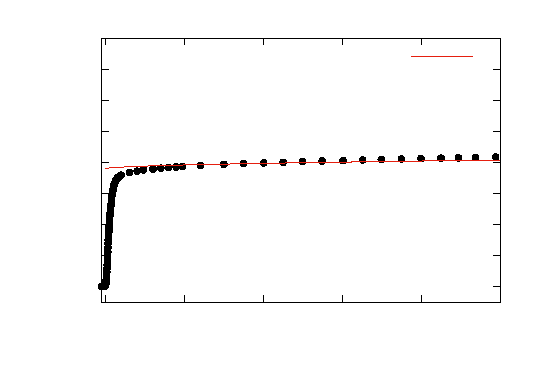
\includegraphics[width={252.00bp},height={172.80bp}]{schotty-1,92A}}%
    \gplfronttext
  \end{picture}%
\endgroup

        \[ I_{\text{nas}} = 37.9 \pm 0.2 \ \mu \text{A} \]
        \caption{ Závislost anodového proudu na anodovém napětí při $ I_f = 1.92 $ A. }
    \end{minipage}
    \hfill
    \begin{minipage}{.45\linewidth}
        \centering
        % GNUPLOT: LaTeX picture with Postscript
\begingroup
  \makeatletter
  \providecommand\color[2][]{%
    \GenericError{(gnuplot) \space\space\space\@spaces}{%
      Package color not loaded in conjunction with
      terminal option `colourtext'%
    }{See the gnuplot documentation for explanation.%
    }{Either use 'blacktext' in gnuplot or load the package
      color.sty in LaTeX.}%
    \renewcommand\color[2][]{}%
  }%
  \providecommand\includegraphics[2][]{%
    \GenericError{(gnuplot) \space\space\space\@spaces}{%
      Package graphicx or graphics not loaded%
    }{See the gnuplot documentation for explanation.%
    }{The gnuplot epslatex terminal needs graphicx.sty or graphics.sty.}%
    \renewcommand\includegraphics[2][]{}%
  }%
  \providecommand\rotatebox[2]{#2}%
  \@ifundefined{ifGPcolor}{%
    \newif\ifGPcolor
    \GPcolorfalse
  }{}%
  \@ifundefined{ifGPblacktext}{%
    \newif\ifGPblacktext
    \GPblacktexttrue
  }{}%
  % define a \g@addto@macro without @ in the name:
  \let\gplgaddtomacro\g@addto@macro
  % define empty templates for all commands taking text:
  \gdef\gplbacktext{}%
  \gdef\gplfronttext{}%
  \makeatother
  \ifGPblacktext
    % no textcolor at all
    \def\colorrgb#1{}%
    \def\colorgray#1{}%
  \else
    % gray or color?
    \ifGPcolor
      \def\colorrgb#1{\color[rgb]{#1}}%
      \def\colorgray#1{\color[gray]{#1}}%
      \expandafter\def\csname LTw\endcsname{\color{white}}%
      \expandafter\def\csname LTb\endcsname{\color{black}}%
      \expandafter\def\csname LTa\endcsname{\color{black}}%
      \expandafter\def\csname LT0\endcsname{\color[rgb]{1,0,0}}%
      \expandafter\def\csname LT1\endcsname{\color[rgb]{0,1,0}}%
      \expandafter\def\csname LT2\endcsname{\color[rgb]{0,0,1}}%
      \expandafter\def\csname LT3\endcsname{\color[rgb]{1,0,1}}%
      \expandafter\def\csname LT4\endcsname{\color[rgb]{0,1,1}}%
      \expandafter\def\csname LT5\endcsname{\color[rgb]{1,1,0}}%
      \expandafter\def\csname LT6\endcsname{\color[rgb]{0,0,0}}%
      \expandafter\def\csname LT7\endcsname{\color[rgb]{1,0.3,0}}%
      \expandafter\def\csname LT8\endcsname{\color[rgb]{0.5,0.5,0.5}}%
    \else
      % gray
      \def\colorrgb#1{\color{black}}%
      \def\colorgray#1{\color[gray]{#1}}%
      \expandafter\def\csname LTw\endcsname{\color{white}}%
      \expandafter\def\csname LTb\endcsname{\color{black}}%
      \expandafter\def\csname LTa\endcsname{\color{black}}%
      \expandafter\def\csname LT0\endcsname{\color{black}}%
      \expandafter\def\csname LT1\endcsname{\color{black}}%
      \expandafter\def\csname LT2\endcsname{\color{black}}%
      \expandafter\def\csname LT3\endcsname{\color{black}}%
      \expandafter\def\csname LT4\endcsname{\color{black}}%
      \expandafter\def\csname LT5\endcsname{\color{black}}%
      \expandafter\def\csname LT6\endcsname{\color{black}}%
      \expandafter\def\csname LT7\endcsname{\color{black}}%
      \expandafter\def\csname LT8\endcsname{\color{black}}%
    \fi
  \fi
    \setlength{\unitlength}{0.0500bp}%
    \ifx\gptboxheight\undefined%
      \newlength{\gptboxheight}%
      \newlength{\gptboxwidth}%
      \newsavebox{\gptboxtext}%
    \fi%
    \setlength{\fboxrule}{0.5pt}%
    \setlength{\fboxsep}{1pt}%
    \definecolor{tbcol}{rgb}{1,1,1}%
\begin{picture}(5040.00,3456.00)%
    \gplgaddtomacro\gplbacktext{%
      \csname LTb\endcsname%%
      \put(682,853){\makebox(0,0)[r]{\strut{}$0$}}%
      \put(682,1151){\makebox(0,0)[r]{\strut{}$10$}}%
      \put(682,1448){\makebox(0,0)[r]{\strut{}$20$}}%
      \put(682,1746){\makebox(0,0)[r]{\strut{}$30$}}%
      \put(682,2044){\makebox(0,0)[r]{\strut{}$40$}}%
      \put(682,2342){\makebox(0,0)[r]{\strut{}$50$}}%
      \put(682,2639){\makebox(0,0)[r]{\strut{}$60$}}%
      \put(682,2937){\makebox(0,0)[r]{\strut{}$70$}}%
      \put(682,3235){\makebox(0,0)[r]{\strut{}$80$}}%
      \put(852,484){\makebox(0,0){\strut{}$0$}}%
      \put(1610,484){\makebox(0,0){\strut{}$100$}}%
      \put(2368,484){\makebox(0,0){\strut{}$200$}}%
      \put(3127,484){\makebox(0,0){\strut{}$300$}}%
      \put(3885,484){\makebox(0,0){\strut{}$400$}}%
      \put(4643,484){\makebox(0,0){\strut{}$500$}}%
    }%
    \gplgaddtomacro\gplfronttext{%
      \csname LTb\endcsname%%
      \put(209,1969){\rotatebox{-270}{\makebox(0,0){\strut{}$ I_a $ ($ \mu $A)  }}}%
      \put(2728,154){\makebox(0,0){\strut{}$ U_a $ (V) }}%
      \csname LTb\endcsname%%
      \put(3656,3062){\makebox(0,0)[r]{\strut{}fit}}%
    }%
    \gplbacktext
    \put(0,0){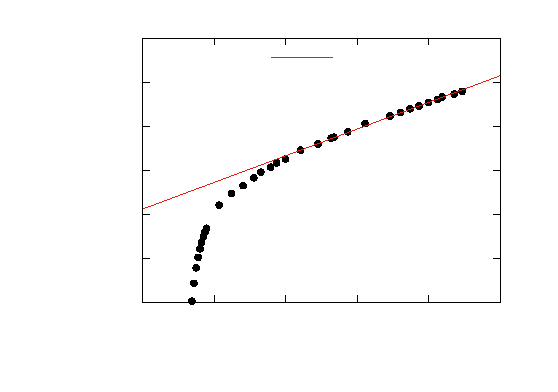
\includegraphics[width={252.00bp},height={172.80bp}]{schotty-1,98A}}%
    \gplfronttext
  \end{picture}%
\endgroup

        \[ I_{\text{nas}} = 63.8 \pm 0.3 \ \mu \text{A} \]
        \caption{Závislost anodového proudu na anodovém napětí při $ I_f = 1.98 $ A }
    \end{minipage}
\end{table}

\vspace{-30pt}

\begin{table}[h]
    \captionsetup{type=graph}
    \begin{minipage}{.45\linewidth}
        \centering
        % GNUPLOT: LaTeX picture with Postscript
\begingroup
  \makeatletter
  \providecommand\color[2][]{%
    \GenericError{(gnuplot) \space\space\space\@spaces}{%
      Package color not loaded in conjunction with
      terminal option `colourtext'%
    }{See the gnuplot documentation for explanation.%
    }{Either use 'blacktext' in gnuplot or load the package
      color.sty in LaTeX.}%
    \renewcommand\color[2][]{}%
  }%
  \providecommand\includegraphics[2][]{%
    \GenericError{(gnuplot) \space\space\space\@spaces}{%
      Package graphicx or graphics not loaded%
    }{See the gnuplot documentation for explanation.%
    }{The gnuplot epslatex terminal needs graphicx.sty or graphics.sty.}%
    \renewcommand\includegraphics[2][]{}%
  }%
  \providecommand\rotatebox[2]{#2}%
  \@ifundefined{ifGPcolor}{%
    \newif\ifGPcolor
    \GPcolorfalse
  }{}%
  \@ifundefined{ifGPblacktext}{%
    \newif\ifGPblacktext
    \GPblacktexttrue
  }{}%
  % define a \g@addto@macro without @ in the name:
  \let\gplgaddtomacro\g@addto@macro
  % define empty templates for all commands taking text:
  \gdef\gplbacktext{}%
  \gdef\gplfronttext{}%
  \makeatother
  \ifGPblacktext
    % no textcolor at all
    \def\colorrgb#1{}%
    \def\colorgray#1{}%
  \else
    % gray or color?
    \ifGPcolor
      \def\colorrgb#1{\color[rgb]{#1}}%
      \def\colorgray#1{\color[gray]{#1}}%
      \expandafter\def\csname LTw\endcsname{\color{white}}%
      \expandafter\def\csname LTb\endcsname{\color{black}}%
      \expandafter\def\csname LTa\endcsname{\color{black}}%
      \expandafter\def\csname LT0\endcsname{\color[rgb]{1,0,0}}%
      \expandafter\def\csname LT1\endcsname{\color[rgb]{0,1,0}}%
      \expandafter\def\csname LT2\endcsname{\color[rgb]{0,0,1}}%
      \expandafter\def\csname LT3\endcsname{\color[rgb]{1,0,1}}%
      \expandafter\def\csname LT4\endcsname{\color[rgb]{0,1,1}}%
      \expandafter\def\csname LT5\endcsname{\color[rgb]{1,1,0}}%
      \expandafter\def\csname LT6\endcsname{\color[rgb]{0,0,0}}%
      \expandafter\def\csname LT7\endcsname{\color[rgb]{1,0.3,0}}%
      \expandafter\def\csname LT8\endcsname{\color[rgb]{0.5,0.5,0.5}}%
    \else
      % gray
      \def\colorrgb#1{\color{black}}%
      \def\colorgray#1{\color[gray]{#1}}%
      \expandafter\def\csname LTw\endcsname{\color{white}}%
      \expandafter\def\csname LTb\endcsname{\color{black}}%
      \expandafter\def\csname LTa\endcsname{\color{black}}%
      \expandafter\def\csname LT0\endcsname{\color{black}}%
      \expandafter\def\csname LT1\endcsname{\color{black}}%
      \expandafter\def\csname LT2\endcsname{\color{black}}%
      \expandafter\def\csname LT3\endcsname{\color{black}}%
      \expandafter\def\csname LT4\endcsname{\color{black}}%
      \expandafter\def\csname LT5\endcsname{\color{black}}%
      \expandafter\def\csname LT6\endcsname{\color{black}}%
      \expandafter\def\csname LT7\endcsname{\color{black}}%
      \expandafter\def\csname LT8\endcsname{\color{black}}%
    \fi
  \fi
    \setlength{\unitlength}{0.0500bp}%
    \ifx\gptboxheight\undefined%
      \newlength{\gptboxheight}%
      \newlength{\gptboxwidth}%
      \newsavebox{\gptboxtext}%
    \fi%
    \setlength{\fboxrule}{0.5pt}%
    \setlength{\fboxsep}{1pt}%
    \definecolor{tbcol}{rgb}{1,1,1}%
\begin{picture}(5040.00,3456.00)%
    \gplgaddtomacro\gplbacktext{%
      \csname LTb\endcsname%%
      \put(814,862){\makebox(0,0)[r]{\strut{}$-24$}}%
      \put(814,1179){\makebox(0,0)[r]{\strut{}$-22$}}%
      \put(814,1495){\makebox(0,0)[r]{\strut{}$-20$}}%
      \put(814,1811){\makebox(0,0)[r]{\strut{}$-18$}}%
      \put(814,2128){\makebox(0,0)[r]{\strut{}$-16$}}%
      \put(814,2444){\makebox(0,0)[r]{\strut{}$-14$}}%
      \put(814,2760){\makebox(0,0)[r]{\strut{}$-12$}}%
      \put(814,3077){\makebox(0,0)[r]{\strut{}$-10$}}%
      \put(1316,484){\makebox(0,0){\strut{}$-4$}}%
      \put(2055,484){\makebox(0,0){\strut{}$-2$}}%
      \put(2795,484){\makebox(0,0){\strut{}$0$}}%
      \put(3534,484){\makebox(0,0){\strut{}$2$}}%
      \put(4273,484){\makebox(0,0){\strut{}$4$}}%
    }%
    \gplgaddtomacro\gplfronttext{%
      \csname LTb\endcsname%%
      \put(209,1969){\rotatebox{-270}{\makebox(0,0){\strut{}$ \log( I_a ) $  }}}%
      \put(2794,154){\makebox(0,0){\strut{}$ U_a $ (V) }}%
      \csname LTb\endcsname%%
      \put(3656,3062){\makebox(0,0)[r]{\strut{}fit}}%
    }%
    \gplbacktext
    \put(0,0){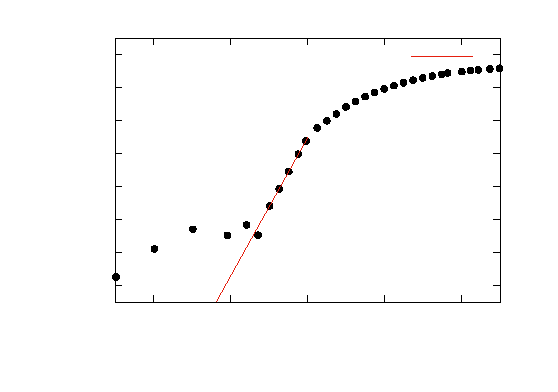
\includegraphics[width={252.00bp},height={172.80bp}]{schotty-1,92A_log}}%
    \gplfronttext
  \end{picture}%
\endgroup

        \[ T = 2654.99 \pm 54.43 \text{ K} \]
        \caption{ Logaritmické závislost anodového proudu na anodovém napětí při $ I_f = 1.92 $ A }
    \end{minipage}
    \hfill
    \begin{minipage}{.45\linewidth}
        \centering
        % GNUPLOT: LaTeX picture with Postscript
\begingroup
  \makeatletter
  \providecommand\color[2][]{%
    \GenericError{(gnuplot) \space\space\space\@spaces}{%
      Package color not loaded in conjunction with
      terminal option `colourtext'%
    }{See the gnuplot documentation for explanation.%
    }{Either use 'blacktext' in gnuplot or load the package
      color.sty in LaTeX.}%
    \renewcommand\color[2][]{}%
  }%
  \providecommand\includegraphics[2][]{%
    \GenericError{(gnuplot) \space\space\space\@spaces}{%
      Package graphicx or graphics not loaded%
    }{See the gnuplot documentation for explanation.%
    }{The gnuplot epslatex terminal needs graphicx.sty or graphics.sty.}%
    \renewcommand\includegraphics[2][]{}%
  }%
  \providecommand\rotatebox[2]{#2}%
  \@ifundefined{ifGPcolor}{%
    \newif\ifGPcolor
    \GPcolorfalse
  }{}%
  \@ifundefined{ifGPblacktext}{%
    \newif\ifGPblacktext
    \GPblacktexttrue
  }{}%
  % define a \g@addto@macro without @ in the name:
  \let\gplgaddtomacro\g@addto@macro
  % define empty templates for all commands taking text:
  \gdef\gplbacktext{}%
  \gdef\gplfronttext{}%
  \makeatother
  \ifGPblacktext
    % no textcolor at all
    \def\colorrgb#1{}%
    \def\colorgray#1{}%
  \else
    % gray or color?
    \ifGPcolor
      \def\colorrgb#1{\color[rgb]{#1}}%
      \def\colorgray#1{\color[gray]{#1}}%
      \expandafter\def\csname LTw\endcsname{\color{white}}%
      \expandafter\def\csname LTb\endcsname{\color{black}}%
      \expandafter\def\csname LTa\endcsname{\color{black}}%
      \expandafter\def\csname LT0\endcsname{\color[rgb]{1,0,0}}%
      \expandafter\def\csname LT1\endcsname{\color[rgb]{0,1,0}}%
      \expandafter\def\csname LT2\endcsname{\color[rgb]{0,0,1}}%
      \expandafter\def\csname LT3\endcsname{\color[rgb]{1,0,1}}%
      \expandafter\def\csname LT4\endcsname{\color[rgb]{0,1,1}}%
      \expandafter\def\csname LT5\endcsname{\color[rgb]{1,1,0}}%
      \expandafter\def\csname LT6\endcsname{\color[rgb]{0,0,0}}%
      \expandafter\def\csname LT7\endcsname{\color[rgb]{1,0.3,0}}%
      \expandafter\def\csname LT8\endcsname{\color[rgb]{0.5,0.5,0.5}}%
    \else
      % gray
      \def\colorrgb#1{\color{black}}%
      \def\colorgray#1{\color[gray]{#1}}%
      \expandafter\def\csname LTw\endcsname{\color{white}}%
      \expandafter\def\csname LTb\endcsname{\color{black}}%
      \expandafter\def\csname LTa\endcsname{\color{black}}%
      \expandafter\def\csname LT0\endcsname{\color{black}}%
      \expandafter\def\csname LT1\endcsname{\color{black}}%
      \expandafter\def\csname LT2\endcsname{\color{black}}%
      \expandafter\def\csname LT3\endcsname{\color{black}}%
      \expandafter\def\csname LT4\endcsname{\color{black}}%
      \expandafter\def\csname LT5\endcsname{\color{black}}%
      \expandafter\def\csname LT6\endcsname{\color{black}}%
      \expandafter\def\csname LT7\endcsname{\color{black}}%
      \expandafter\def\csname LT8\endcsname{\color{black}}%
    \fi
  \fi
    \setlength{\unitlength}{0.0500bp}%
    \ifx\gptboxheight\undefined%
      \newlength{\gptboxheight}%
      \newlength{\gptboxwidth}%
      \newsavebox{\gptboxtext}%
    \fi%
    \setlength{\fboxrule}{0.5pt}%
    \setlength{\fboxsep}{1pt}%
    \definecolor{tbcol}{rgb}{1,1,1}%
\begin{picture}(5040.00,3456.00)%
    \gplgaddtomacro\gplbacktext{%
      \csname LTb\endcsname%%
      \put(814,862){\makebox(0,0)[r]{\strut{}$-24$}}%
      \put(814,1179){\makebox(0,0)[r]{\strut{}$-22$}}%
      \put(814,1495){\makebox(0,0)[r]{\strut{}$-20$}}%
      \put(814,1811){\makebox(0,0)[r]{\strut{}$-18$}}%
      \put(814,2128){\makebox(0,0)[r]{\strut{}$-16$}}%
      \put(814,2444){\makebox(0,0)[r]{\strut{}$-14$}}%
      \put(814,2760){\makebox(0,0)[r]{\strut{}$-12$}}%
      \put(814,3077){\makebox(0,0)[r]{\strut{}$-10$}}%
      \put(1316,484){\makebox(0,0){\strut{}$-4$}}%
      \put(2055,484){\makebox(0,0){\strut{}$-2$}}%
      \put(2795,484){\makebox(0,0){\strut{}$0$}}%
      \put(3534,484){\makebox(0,0){\strut{}$2$}}%
      \put(4273,484){\makebox(0,0){\strut{}$4$}}%
    }%
    \gplgaddtomacro\gplfronttext{%
      \csname LTb\endcsname%%
      \put(209,1969){\rotatebox{-270}{\makebox(0,0){\strut{}$ \log( I_a ) $  }}}%
      \put(2794,154){\makebox(0,0){\strut{}$ U_a $ (V) }}%
      \csname LTb\endcsname%%
      \put(3656,3062){\makebox(0,0)[r]{\strut{}fit}}%
    }%
    \gplbacktext
    \put(0,0){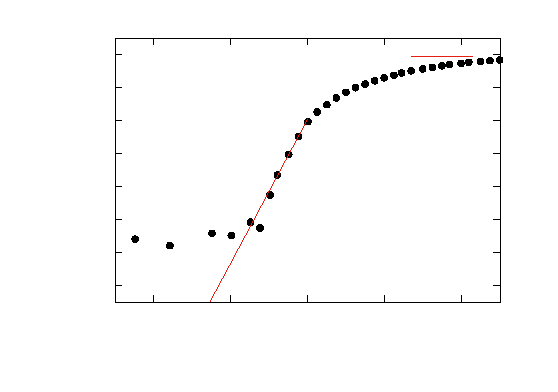
\includegraphics[width={252.00bp},height={172.80bp}]{schotty-1,98A_log}}%
    \gplfronttext
  \end{picture}%
\endgroup

        \[ T = 2764.03 \pm 8.108 \text{ K} \]

        \caption{Logaritmické závislost anodového proudu na anodovém napětí při $ I_f = 1.98 $ A }
    \end{minipage}
\end{table}

\subsection{Závislost nasyceného proudu na žhavícím proudu}

Při obou měřených žhavících proudech došlo k ustálení anodového proudu kolem $ U_a = 20 $ V, takže závislost $ I_{\text{nas}} = f(T(I_f, U_f)) $ budu měřit při tomto napětí. Pokaždé když změním žhavící napětí je opět potřeba nějakou dobu počkat na zahřátí čidla a proto změřených hodnot není tolik. Teplotu jsem ze žhavícího napětí a proudu spočítal podle vztahu (9) a výstupní práci zjistím fitem zlogaritmovanéhé Richardson – Dushmanovy rovnice (8)

\begin{equation*}
w = 4.04 \pm 0.09 \text{ (eV)}
\end{equation*}

\begin{figure}[h]
    \centering
    % GNUPLOT: LaTeX picture with Postscript
\begingroup
  \makeatletter
  \providecommand\color[2][]{%
    \GenericError{(gnuplot) \space\space\space\@spaces}{%
      Package color not loaded in conjunction with
      terminal option `colourtext'%
    }{See the gnuplot documentation for explanation.%
    }{Either use 'blacktext' in gnuplot or load the package
      color.sty in LaTeX.}%
    \renewcommand\color[2][]{}%
  }%
  \providecommand\includegraphics[2][]{%
    \GenericError{(gnuplot) \space\space\space\@spaces}{%
      Package graphicx or graphics not loaded%
    }{See the gnuplot documentation for explanation.%
    }{The gnuplot epslatex terminal needs graphicx.sty or graphics.sty.}%
    \renewcommand\includegraphics[2][]{}%
  }%
  \providecommand\rotatebox[2]{#2}%
  \@ifundefined{ifGPcolor}{%
    \newif\ifGPcolor
    \GPcolorfalse
  }{}%
  \@ifundefined{ifGPblacktext}{%
    \newif\ifGPblacktext
    \GPblacktexttrue
  }{}%
  % define a \g@addto@macro without @ in the name:
  \let\gplgaddtomacro\g@addto@macro
  % define empty templates for all commands taking text:
  \gdef\gplbacktext{}%
  \gdef\gplfronttext{}%
  \makeatother
  \ifGPblacktext
    % no textcolor at all
    \def\colorrgb#1{}%
    \def\colorgray#1{}%
  \else
    % gray or color?
    \ifGPcolor
      \def\colorrgb#1{\color[rgb]{#1}}%
      \def\colorgray#1{\color[gray]{#1}}%
      \expandafter\def\csname LTw\endcsname{\color{white}}%
      \expandafter\def\csname LTb\endcsname{\color{black}}%
      \expandafter\def\csname LTa\endcsname{\color{black}}%
      \expandafter\def\csname LT0\endcsname{\color[rgb]{1,0,0}}%
      \expandafter\def\csname LT1\endcsname{\color[rgb]{0,1,0}}%
      \expandafter\def\csname LT2\endcsname{\color[rgb]{0,0,1}}%
      \expandafter\def\csname LT3\endcsname{\color[rgb]{1,0,1}}%
      \expandafter\def\csname LT4\endcsname{\color[rgb]{0,1,1}}%
      \expandafter\def\csname LT5\endcsname{\color[rgb]{1,1,0}}%
      \expandafter\def\csname LT6\endcsname{\color[rgb]{0,0,0}}%
      \expandafter\def\csname LT7\endcsname{\color[rgb]{1,0.3,0}}%
      \expandafter\def\csname LT8\endcsname{\color[rgb]{0.5,0.5,0.5}}%
    \else
      % gray
      \def\colorrgb#1{\color{black}}%
      \def\colorgray#1{\color[gray]{#1}}%
      \expandafter\def\csname LTw\endcsname{\color{white}}%
      \expandafter\def\csname LTb\endcsname{\color{black}}%
      \expandafter\def\csname LTa\endcsname{\color{black}}%
      \expandafter\def\csname LT0\endcsname{\color{black}}%
      \expandafter\def\csname LT1\endcsname{\color{black}}%
      \expandafter\def\csname LT2\endcsname{\color{black}}%
      \expandafter\def\csname LT3\endcsname{\color{black}}%
      \expandafter\def\csname LT4\endcsname{\color{black}}%
      \expandafter\def\csname LT5\endcsname{\color{black}}%
      \expandafter\def\csname LT6\endcsname{\color{black}}%
      \expandafter\def\csname LT7\endcsname{\color{black}}%
      \expandafter\def\csname LT8\endcsname{\color{black}}%
    \fi
  \fi
    \setlength{\unitlength}{0.0500bp}%
    \ifx\gptboxheight\undefined%
      \newlength{\gptboxheight}%
      \newlength{\gptboxwidth}%
      \newsavebox{\gptboxtext}%
    \fi%
    \setlength{\fboxrule}{0.5pt}%
    \setlength{\fboxsep}{1pt}%
    \definecolor{tbcol}{rgb}{1,1,1}%
\begin{picture}(5328.00,3600.00)%
    \gplgaddtomacro\gplbacktext{%
      \csname LTb\endcsname%%
      \put(814,704){\makebox(0,0)[r]{\strut{}$-36$}}%
      \put(814,1086){\makebox(0,0)[r]{\strut{}$-34$}}%
      \put(814,1468){\makebox(0,0)[r]{\strut{}$-32$}}%
      \put(814,1850){\makebox(0,0)[r]{\strut{}$-30$}}%
      \put(814,2233){\makebox(0,0)[r]{\strut{}$-28$}}%
      \put(814,2615){\makebox(0,0)[r]{\strut{}$-26$}}%
      \put(814,2997){\makebox(0,0)[r]{\strut{}$-24$}}%
      \put(814,3379){\makebox(0,0)[r]{\strut{}$-22$}}%
      \put(946,484){\makebox(0,0){\strut{}$0.00065$}}%
      \put(1743,484){\makebox(0,0){\strut{}$0.0007$}}%
      \put(2540,484){\makebox(0,0){\strut{}$0.00075$}}%
      \put(3337,484){\makebox(0,0){\strut{}$0.0008$}}%
      \put(4134,484){\makebox(0,0){\strut{}$0.00085$}}%
      \put(4931,484){\makebox(0,0){\strut{}$0.0009$}}%
    }%
    \gplgaddtomacro\gplfronttext{%
      \csname LTb\endcsname%%
      \put(209,2041){\rotatebox{-270}{\makebox(0,0){\strut{} $ \log(I_a/T^2) $ }}}%
      \put(2938,154){\makebox(0,0){\strut{} $ 1/T $ (K$^{-1} $) }}%
      \csname LTb\endcsname%%
      \put(3944,3206){\makebox(0,0)[r]{\strut{}fit}}%
    }%
    \gplbacktext
    \put(0,0){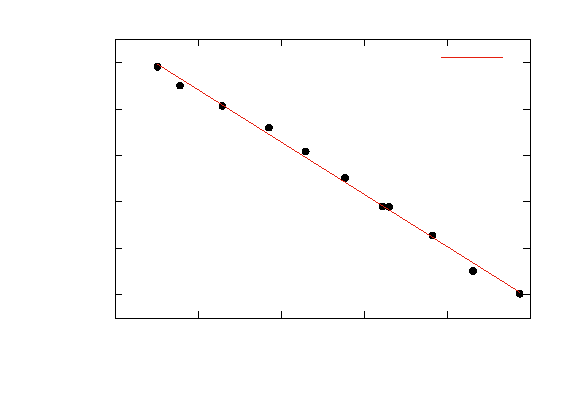
\includegraphics[width={266.40bp},height={180.00bp}]{teplota}}%
    \gplfronttext
  \end{picture}%
\endgroup

    \caption{Závislost anodového proudu na teplotě katody }
\end{figure}

\section{Závěr}

Povedlo se ověřit vztah (12), který popisuje Schottkyho efekt. Při přivedení elektrického pole na wolframovou katodu došlo ke snížení výstupní práce elektronů a většímu nasycenému proudu přibližně podle tohoto vztahu. 

V druhé části jsem ověřil Richardson – Dushmanovu rovnice (8) popisující nasycený proud v závislosti na rostoucí teplotě a z fitu naměřených dat zjistil výstupní práci wolframu $ w = 4.04 \pm 0.09 \text{ (eV)} $. Tabulková hodnota udává $ w = 4.5  \text{ (eV)} $


\begin{thebibliography}{0}
\bibitem{tabulky} Hustota pevných látek. Dostupné z~\url{http://www.converter.cz/tabulky/hustota-pevne.htmf}.   
\end{thebibliography}

\end{document}
